%{{第六十九回}}{第六十九回}}

\chapter{弄小巧用借剑杀人\\觉大限吞生金自逝}
{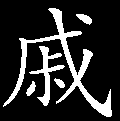
\includegraphics[width=3mm]{../Images/00005}\kaishu      写凤姐写不尽,却从上下左右写。写秋桐极淫邪,正写凤姐极淫邪;写平儿极义气,正写凤姐极不义气;写使女欺压二姐,正写凤姐欺压二姐;写下人感戴二姐,正写下人不感戴凤姐。史公用意,非念死书子之所知。}

话说尤二姐听了,又感谢不尽,只得跟了他来。尤氏那边怎好不过来的,少不得也过来跟着凤姐去回,方是大礼。凤姐笑说:``你只别说话,等我去说。''尤氏道:``这个自然。但一有个不是,是往你身上推的。''说着,大家先来至贾母房中。

正值贾母和园中姊妹们说笑解闷,忽见凤姐带了一个标致小媳妇进来,忙觑着眼看,说:``这是谁家的孩子!好可怜见的。''凤姐上来笑道:``老祖宗倒细细的看看,好不好?''说着,忙拉二姐说:``这是太婆婆,快磕头。''二姐忙行了大礼,展拜起来。又指着众姊妹说:这是某人某人,你先认了,太太瞧过了再见礼。二姐听了,一一又从新故意的问过,垂头站在旁边。贾母上下瞧了一遍,因又笑问:``你姓什么?今年十几了?''凤姐忙又笑说:``老祖宗且别问,只说比我俊不俊。''贾母又戴了眼镜,命鸳鸯琥珀:``把那孩子拉过来,我瞧瞧肉皮儿。''众人都抿嘴儿笑着,只得推他上去。贾母细瞧了一遍,又命琥珀:``拿出手来我瞧瞧。''鸳鸯又\elegantpar{揭起裙子来}{看脚,是天足,齐全孩子}。贾母瞧毕,摘下眼镜来,笑说道:``更是个齐全孩子,我看比你俊些。''凤姐听说,笑着忙跪下,将尤氏那边所编之话,一五一十细细的说了一遍,``少不得老祖宗发慈心,先许他进来,住一年后再圆房。''贾母听了道:``这有什么不是。既你这样贤良,很好。只是一年后方可圆得房。''凤姐听了,叩头起来,又求贾母着两个女人一同带去见太太们,说是老祖宗的主意。贾母依允,遂使二人带去见了邢夫人等。王夫人正因他风声不雅,深为忧虑,见他今行此事,岂有不乐之理。于是尤二姐自此见了天日,挪到厢房住居。

凤姐一面使人暗暗调唆张华,只叫他要原妻,这里还有许多赔送外,还给他银子安家过活。张华原无胆无心告贾家的,后来又见贾蓉打发人来对词,那人原说的:``张华先退了亲。我们皆是亲戚。接到家里住着是真,并无婚娶之说。皆因张华拖欠了我们的债务,追索不与,方诬赖小的主人那些个。''察院都和贾王两处有瓜葛,况又受了贿,只说张华无赖,以穷讹诈,状子也不收,打了一顿赶出来。庆儿在外替他打点,也没打重。又调唆张华:``亲原是你家定的,你只要亲事,官必还断给你。''于是又告。王信那边又透了消息与察院,察院便批:``张华所欠贾宅之银,令其限内按数交还,其所定之亲,仍令其有力时娶回。''又传了他父亲来当堂批准。他父亲亦系庆儿说明,乐得人财两进,便去贾家领人。

凤姐儿一面吓的来回贾母,说如此这般,都是珍大嫂子干事不明,并没和那家退准,惹人告了,如此官断。贾母听了,忙唤了尤氏过来,说他作事不妥,``既是你妹子从小曾与人指腹为婚,又没退断,使人混告了。''尤氏听了,只得说:``他连银子都收了,怎么没准。''凤姐在旁又说:``张华的口供上现说不曾见银子,也没见人去。他老子说:`原是亲家母说过一次,并没应准。亲家母死了,你们就接进去作二房。'如此没有对证,只好由他去混说。幸而琏二爷不在家,没曾圆房,这还无妨。只是人已来了,怎好送回去,岂不伤脸。''贾母道:``又没圆房,没的强占人家有夫之人,名声也不好,不如送给他去。那里寻不出好人来。''尤二姐听了,又回贾母说:``我母亲实于某年月日给了他十两银子退准的。他因穷急了告,又翻了口。我姐姐原没错办。''贾母听了,便说:``可见刁民难惹。既这样,凤丫头去料理料理。''凤姐听了无法,只得应着。回来只命人去找贾蓉。

贾蓉深知凤姐之意,若要使张华领回,成何体统,便回了贾珍,暗暗遣人去说张华:``你如今既有许多银子,何必定要原人。若只管执定主意,岂不怕爷们一怒,寻出个由头,你死无葬身之地。你有了银子,回家去什么好人寻不出来。你若走时,还赏你些路费。''张华听了,心中想了一想,这倒是好主意,和父亲商议已定,约共也得了有百金,父子次日起个五更,回原籍去了。贾蓉打听得真了,来回了贾母凤姐,说:``张华父子妄告不实,惧罪逃走,官府亦知此情,也不追究,大事完毕。''凤姐听了,心中一想:若必定着张华带回二姐去,未免贾琏回来再花几个钱包占住,不怕张华不依。还是二姐不去,自己相伴着还妥当,且再作道理。只是张华此去不知何往,他倘或再将此事告诉了别人,或日后再寻出这由头来翻案,岂不是自己害了自己。原先不该如此将刀靶付与外人去的。因此悔之不迭,复又想了一条主意出来,悄命旺儿遣人寻着了他,或说他作贼,和他打官司将他治死;或暗中使人算计,务将张华治死,方剪草除根,保住自己的名誉。旺儿领命出来,回家细想:人已走了完事,何必如此大作,人命关天,非同儿戏,我且哄过他去,再作道理。因此在外躲了几日,回来告诉凤姐,只说张华是有了几两银子在身上,逃去第三日在京口地界五更天已被截路人打闷棍打死了。他老子唬死在店房,在那里验尸掩埋。凤姐听了不信,说:``你要扯谎,我再使人打听出来敲你的牙!''自此方丢过不究。凤姐和尤二姐和美非常,更比\elegantpar{亲姊亲妹}{既是赚入,那是上了梁山了}还胜十倍。

那贾琏一日事毕回来,先到了新房中,已竟悄悄的封锁,只有一个看房子的老头儿。贾琏问他原故,老头子细说原委,贾琏只在镫中跌足。少不得来见贾赦与邢夫人,将所完之事回明。贾赦十分欢喜,说他中用,赏了他一百两银子,又将房中一个十七岁的丫鬟名唤秋桐者,赏他为妾。贾琏叩头领去,喜之不尽。见了贾母和家中人,回来见凤姐,未免脸上有些愧色。谁知凤姐儿他反不似往日容颜,同尤二姐一同出迎,叙了寒温。贾琏将秋桐之事说了,未免脸上有些得意之色,骄矜之容。凤姐听了,忙命两个媳妇坐车在那边接了来。心中一刺未除,又平空添了一刺,说不得且吞声忍气,将好颜面换出来遮掩。一面又命摆酒接风,一面带了秋桐来见贾母与王夫人等。贾琏心中也暗暗的纳罕。

那日已是腊月十二日,贾珍起身,先拜了宗祠,然后过来辞拜贾母等人。和族中人直送到洒泪亭方回,独贾琏贾蓉二人送出三日三夜方回。一路上贾珍命他好生收心治家等语,二人口内答应,也说些大礼套话,不必烦叙。

且说凤姐在家,外面待尤二姐自不必说得,只是心中又怀别意。无人处只和尤二姐说:``妹妹的声名很不好听,连老太太、太太们都知道了,说妹妹在家做女孩儿就不干净,又和姐夫有些首尾,`没人要的了你拣了来,还不休了再寻好的。'我听见这话,气得倒仰,查是谁说的,又查不出来。这日久天长,这些个奴才们跟前,怎么说嘴。我反弄了个鱼头来拆。''说了两遍,自己又气病了,茶饭也不吃,除了平儿,众丫头媳妇无不言三语四,指桑说槐,暗相讥刺。秋桐自为系贾赦之赐,无人僭他的,连凤姐平儿皆不放在眼里,岂肯容他。张口是``先奸后娶没汉子要的娼妇,也来要我的强。''凤姐听了暗乐,尤二姐听了暗愧暗怒暗气。凤姐既装病,便不和尤二姐吃饭了。每日只命人端了菜饭到他房中去吃,那茶饭都系不堪之物。平儿看不过,自拿了钱出来弄菜与他吃,或是有时只说和他园中去顽,在园中厨内另做了汤水与他吃,也无人敢回凤姐。只有秋桐一时撞见了,便去说舌告诉凤姐说:``奶奶的名声,生是平儿弄坏了的。这样好菜好饭浪着不吃,却往园里去偷吃。''凤姐听了,骂平儿说:``人家养猫拿耗子,我的猫只倒咬鸡。''平儿不敢多说,自此也要远着了。又暗恨秋桐,难以出口。

园中姊妹如李纨、迎春、惜春等人,皆为凤姐是好意,然宝、黛一干人暗为二姐担心。虽都不便多事,惟见二姐可怜,常来了,倒还都悯恤他。每日常无人处说起话来,尤二姐便淌眼抹泪,又不敢抱怨。凤姐儿又并无露出一点坏形来。贾琏来家时,见了凤姐贤良,也便不留心。况素习以来因贾赦姬妾丫鬟最多,贾琏每怀不轨之心,只未敢下手。如这秋桐辈等人,皆是恨老爷年迈昏愦,贪多嚼不烂,没的留下这些人作什么,因此除了几个知礼有耻的,馀者或有与二门上小幺儿们嘲戏的。甚至于与贾琏眉来眼去相偷期的,只惧贾赦之威,未曾到手。这秋桐便和贾琏有旧,从未来过一次。今日天缘凑巧,竟赏了他,真是一对烈火干柴,\elegantpar{如胶投漆}{这漆是万用},燕尔新婚,连日那里拆的开。那贾琏在二姐身上之心也渐渐淡了,只有秋桐一人是命。凤姐虽恨秋桐,且喜借他先可发脱二姐,自己且抽头,用``借剑杀人''之法,``坐山观虎斗'',等秋桐杀了尤二姐,自己再杀秋桐。主意已定,没人处常又私劝秋桐说:``你年轻不知事。他现是二房奶奶,你爷心坎儿上的人,我还让他三分,你去硬碰他,岂不是自寻其死?''那秋桐听了这话,越发恼了,天天大口乱骂说:``奶奶是软弱人,那等贤惠,我却做不来。奶奶把素日的威风怎都没了。奶奶宽洪大量,我却眼里揉不下沙子去。让我和他这淫妇做一回,他才知道。''凤姐儿在屋里,只装不敢出声儿。气的尤二姐在房里哭泣,饭也不吃,又不敢告诉贾琏。次日贾母见他眼红红的肿了,问他,又不敢说。秋桐正是抓乖卖俏之时,他便悄悄的告诉贾母王夫人等说:``专会作死,好好的成天家号丧,背地里咒二奶奶和我早死了,他好和二爷一心一计的过。''贾母听了便说:``人太生娇俏了,可知心就嫉妒。凤丫头倒好意待他,他倒这样争锋吃醋的。可是个贱骨头。''因此渐次便不大喜欢。众人见贾母不喜,不免又往下踏践起来,弄得这尤二姐要死不能,要生不得。还是亏了平儿,时常背着凤姐,看他这般,与他排解排解。

那尤二姐原是个花为肠肚雪作肌肤的人,如何经得这般磨折,不过受了一个月的暗气,便恹恹得了一病,四肢懒动,茶饭不进,渐次黄瘦下去。夜来合上眼,只见他小妹子手捧鸳鸯宝剑前来说:``姐姐,你一生为人心痴意软,终吃了这亏。休信那妒妇花言巧语,外作贤良,内藏奸狡,他发恨定要弄你一死方休。若妹子在世,断不肯令你进来,即进来时,亦不容他这样。此亦系理数应然,你我生前淫奔不才,使人家丧伦败行,故有此报。你依我将此剑斩了那妒妇,一同归至警幻案下,听其发落。不然,你则白白的丧命,且无人怜惜。''尤二姐泣道:``妹妹,我一生品行既亏,今日之报既系当然,何必又生杀戮之冤。随我去忍耐。若天见怜,使我好了,岂不两全。''小妹笑道:``姐姐,你终是个痴人。自古`天网恢恢,疏而不漏',天道好还。你虽悔过自新,然\elegantpar{已将人父子兄弟致于}{又是妲己说}麀聚之乱,天怎容你安生。''尤二姐泣道:``既不得安生,亦是理之当然,奴亦无怨。''小妹听了,长叹而去。尤二姐惊醒,却是一梦。等贾琏来看时,因无人在侧,便泣说:``我这病便不能好了。我来了半年,腹中也有身孕,但不能预知男女。倘天见怜,生了下来还可,若不然,我这命就不保,何况于他。''贾琏亦泣说:``你只放心,我请明人来医治。''于是出去即刻请医生。

谁知王太医亦谋干了军前效力,回来好讨荫封的。小厮们走去,便请了个姓胡的太医,名叫君荣。进来诊脉看了,说是经水不调,全要大补。贾琏便说:``已是三月庚信不行,又常作呕酸,恐是胎气。''胡君荣听了,复又命老婆子们请出手来再看看。尤二姐少不得又从帐内伸出手来。胡君荣又诊了半日,说:``若论胎气,肝脉自应洪大。然木盛则生火,经水不调亦皆因由肝木所致。医生要大胆,须得请奶奶将金面略露露,医生观观气色,方敢下药。''贾琏无法,只得命将帐子掀起一缝,尤二姐露出脸来。胡君荣一见,魂魄如飞上九天,通身麻木,一无所知。一时掩了帐子,贾琏就陪他出来,问是如何。胡太医道:``不是胎气,只是瘀血凝结。如今只以下瘀血通经脉要紧。''于是写了一方,作辞而去。

贾琏命人送了药礼,抓了药来,调服下去。只半夜,尤二姐腹痛不止,谁知竟将一个已成形的男胎打了下来。于是血行不止,二姐就昏迷过去。贾琏闻知,大骂胡君荣。一面再遣人去请医调治,一面命人去打告胡君荣。胡君荣听了,早已卷包逃走。这里太医便说:``本来气血生成亏弱,受胎以来,想是着了些气恼,郁结于中。这位先生擅用虎狼之剂,如今大人元气十分伤其八九,一时难保就愈。煎丸二药并行,还要一些闲言闲事不闻,庶可望好。''说毕而去。急的贾琏查是谁请了姓胡的来,一时查了出来,便打了半死。凤姐比贾琏更急十倍,只说:``咱们命中无子,好容易有了一个,又遇见这样没本事的大夫。''于是天地前烧香礼拜,自己通陈祷告说:``我或有病,只求尤氏妹子身体大愈,再得怀胎生一男子,我愿吃长斋念佛。''贾琏众人见了,无不称赞。贾琏与秋桐在一处时,凤姐又做汤做水的着人送与二姐。又骂平儿不是个有福的,``也和我一样。我因多病了,你却无病也不见怀胎。如今二奶奶这样,都因咱们无福,或犯了什么,冲的他这样。''因又叫人出去算命打卦。偏算命的回来又说:``系属兔的阴人冲犯。''大家算将起来,只有秋桐一人属兔,说他冲的。

秋桐近见贾琏请医治药,打人骂狗,为尤二姐十分尽心,他心中早浸了一缸醋在内了。今又听见如此说他冲了,凤姐儿又劝他说:``你暂且别处去躲几个月再来。''秋桐便气的哭骂道:``理那起瞎肏的混咬舌根!我和他`井水不犯河水',怎么就冲了他!好个爱八哥儿,在外头什么人不见,偏来了就有人冲了。白眉赤脸,那里来的孩子?他不过指着哄我们那个棉花耳朵的爷罢了。纵有孩子,也不知姓张姓王。奶奶希罕那杂种羔子,我不喜欢!老了谁不成?谁不会养!一年半载养一个,倒还是一点搀杂没有的呢!''骂的众人又要笑,又不敢笑。可巧邢夫人过来请安,秋桐便哭告邢夫人说:``二爷奶奶要撵我回去,我没了安身之处,太太好歹开恩。''邢夫人听说,慌的数落凤姐儿一阵,又骂贾琏:``不知好歹的种子,凭他怎不好,是你父亲给的。为个外头来的撵他,连老子都没了。你要撵他,你不如还你父亲去倒好。''说着,赌气去了。秋桐更又得意,越性走到他窗户根底下大哭大骂起来。尤二姐听了,不免更添烦恼。

晚间,贾琏在秋桐房中歇了,凤姐已睡,平儿过来瞧他,又悄悄劝他:``好生养病,不要理那畜生。''尤二姐拉他哭道:``姐姐,我从到了这里,多亏姐姐照应。为我,姐姐也不知受了多少闲气。我若逃的出命来,我必答报姐姐的恩德,只怕我逃不出命来,也只好等来生罢。''平儿也不禁滴泪说道:``想来都是我坑了你。我原是一片痴心,从没瞒他的话。既听见你在外头,岂有不告诉他的。谁知生出这些个事来。''尤二姐忙道:``姐姐这话错了。若姐姐便不告诉他,他岂有打听不出来的,不过是姐姐说的在先。况且我也要一心进来,方成个体统,与姐姐何干。''二人哭了一回,平儿又嘱咐了几句,夜已深了,方去安息。

这里尤二姐心下自思:``病已成势,日无所养,反有所伤,料定必不能好。况胎已打下,无可悬心,何必受这些零气,不如一死,倒还干净。常听见人说,生金子可以坠死,岂不比上吊自刎又干净。''想毕,拃挣起来,打开箱子,找出一块生金,也不知多重,恨命含泪便吞入口中,几次狠命直脖,方咽了下去。于是赶忙将衣服首饰穿戴齐整,上炕躺下了。当下人不知,鬼不觉。到第二日早晨,丫鬟媳妇们见他不叫人,乐得且自己去梳洗。凤姐便和秋桐都上去了。平儿看不过,说丫头们:``你们就只配没人心的打着骂着使也罢了,一个病人,也不知可怜可怜。他虽好性儿,你们也该拿出个样儿来,别太过逾了,墙倒众人推。''丫鬟听了,急推房门进来看时,却穿戴的齐齐整整,死在炕上。于是方吓慌了,喊叫起来。平儿进来看了,不禁大哭。众人虽素习惧怕凤姐,然想尤二姐实在温和怜下,比凤姐原强,如今死去,谁不伤心落泪,只不敢与凤姐看见。

当下合宅皆知。贾琏进来,搂尸大哭不止。凤姐也假意哭:``狠心的妹妹!你怎么丢下我去了,辜负了我的心!''尤氏贾蓉等也来哭了一场,劝住贾琏。贾琏便回了王夫人,讨了梨香院停放五日,挪到铁槛寺去,王夫人依允。贾琏忙命人去开了梨香院的门,收拾出正房来停灵。贾琏嫌后门出灵不像,便对着梨香院的正墙上通街现开了一个大门。两边搭棚,安坛场做佛事。用软榻铺了锦缎衾褥,将二姐抬上榻去,用衾单盖了。八个小厮和几个媳妇围随,从内子墙一带抬往梨香院来。那里已请下天文生预备,揭起衾单一看,只见这尤二姐面色如生,比活着还美貌。贾琏又搂着大哭,只叫``奶奶,你死的不明,都是我坑了你!''贾蓉忙上来劝:``叔叔解着些儿,我这个姨娘自己没福。''说着,又向南指大观园的界墙,贾琏会意,只悄悄跌脚说:``我忽略了,终久对出来,我替你报仇。''天文生回说:``奶奶卒于今日正卯时,五日出不得,或是三日,或是七日方可。明日寅时入殓大吉。''贾琏道:``三日断乎使不得,竟是七日。因家叔家兄皆在外,小丧不敢多停,等到外头,还放五七,做大道场才掩灵。明年往南去下葬。''天文生应诺,写了殃榜而去。宝玉已早过来陪哭一场。众族中人也都来了。

贾琏忙进去,找凤姐要银子治办棺椁丧礼。凤姐见抬了出去,推有病,回:``老太太、太太说我病着,忌三房,不许我去。''因此也不出来穿孝,且往大观园中来。绕过群山,至北界墙根下往外听,隐隐绰绰听了一言半语,回来又回贾母说如此这般。贾母道:``信他胡说,谁家痨病死的孩子不烧了一撒,也认真的开丧破土起来。既是二房一场,也是夫妻之分,停五七日抬出来,或一烧或乱葬地上埋了完事。''凤姐笑道:``可是这话。我又不敢劝他。''正说着,丫鬟来请凤姐,说:``二爷等着奶奶拿银子呢。''凤姐只得来了,便问他``什么银子?家里近来艰难,你还不知道?咱们的月例,一月赶不上一月,鸡儿吃了过年粮。昨儿我把两个金项圈当了三百银子,你还做梦呢。这里还有二三十两银子,你要就拿去。''说着,命平儿拿了出来,递与贾琏,指着贾母有话,又去了。恨的贾琏没话可说,只得开了尤氏箱柜,去拿自己的梯己。及开了箱柜,一滴无存,只有些折簪烂花并几件半新不旧的绸绢衣裳,都是尤二姐素习所穿的,不禁又伤心哭了起来。自己用个包袱一齐包了,也不命小丫鬟来拿,便自己提着来烧。

平儿又是伤心,又是好笑,忙将二百两一包的碎银子偷了出来,到厢房拉住贾琏,悄递与他说:``你只别作声才好,你要哭,外头多少哭不得,又跑了这里来点眼。''贾琏听说,便说:``你说的是。''接了银子,又将一条裙子递与平儿,说:``这是他家常穿的,你好生替我收着,作个念心儿。''平儿只得掩了,自己收去。贾琏拿了银子与衣服,走来命人先去买板。\elegantpar{好的又贵,中的又不要。}{怎样评价红楼梦中,尤二姐和尤三姐二人呢?$zhihu.com/question/31335873/answer/233288886$,偏有人就浪荡子也有真情,为秦可卿的棺材,为二姐的棺材,就谅了贾珍贾琏。}贾琏骑马自去要瞧,至晚间果抬了一副好板进来,价银五百两赊着,连夜赶造。一面分派了人口穿孝守灵,晚来也不进去,只在这里伴宿。正是------

{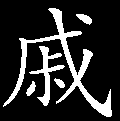
\includegraphics[width=3mm]{../Images/00005}\kaishu 总评:凤姐初念在张华领出二姐,转念又恐仍为外宅,转念即欲杀张华,为斩草除根计。一时写来,觉满腔都是荆棘,浑身都是爪牙,安得借鸳鸯剑手刃其首,以寒千古奸妇之胆。}

{\kaishu 看三姐梦中相叙一段,真有孝子悌弟、义士忠臣之慨,我不禁泪流一斗,湿地三尺。}
